\documentclass{beamer}

% \usepackage{beamerthemesplit} // Activate for custom appearance

\title{Multiple Regression}
\author{Frank Wood}
%\date{\today}

\newcommand{\comment}[1]{}
\newcommand{\ponedec}{\mathcal{P}^\downarrow_1}
\newcommand{\pone}{\mathcal{P}_1}
\newcommand{\rank}[1]{\mathrm{RANK}\left[#1\right]}
\newcommand{\E}[1]{\mathrm{E}\left[#1\right]}
\newcommand{\py}{\mathcal{PY}}
\newcommand{\iid}{iid.}
\newcommand{\drawiid}{\stackrel{\text{iid}}{\sim}}
\newcommand{\vect}[1]{\mathbf{#1}}
\newcommand{\indicator}[1]{\text{I}\left[ #1 \right]}
\newcommand{\pdcoag}{PD(d_1,0)-\text{COAG}}
\newcommand{\todo}{\textbf{*TODO*}}
\newcommand{\igram}{\text{$\infty$-gram}}
\newcommand{\Prob}{\text{P}}

\def\mm{sequence memoizer }
\def\MM{SM }

\def\pibf{{\boldsymbol{\pi}}}
\def\kapbf{\boldsymbol{\kappa}}
\def\taubf{\boldsymbol{\tau}}
\def\thebf{\boldsymbol{\theta}}
\def\rhobf{\boldsymbol{\rho}}
\def\phibf{\boldsymbol{\phi}}
\def\pbf{\mathbf{p}}
\def\qbf{\mathbf{q}}
\def\sbf{\mathbf{s}}
\def\tbf{\mathbf{t}}
\def\ebf{\mathbf{e}}
\def\ybf{\mathbf{y}}
\def\wbf{\mathbf{w}}
\def\xbf{\mathbf{x}}
\def\rbf{\mathbf{r}}
\def\tbf{\mathbf{t}}
\def\kbf{\mathbf{k}}
\def\Xbf{\mathbf{X}}
\def\Abf{\mathbf{A}}
\def\Jbf{\mathbf{J}}
\def\ybf{\mathbf{Y}}
\def\Hbf{\mathbf{H}}
\def\Ibf{\mathbf{I}}
\def\ybf{\mathbf{y}}
\def\bbf{\mathbf{b}}
\def\0bf{\mathbf{0}}
\def\Ibf{\mathbf{I}}
\def\phibf{\mathbf{\phi}}
\def\Phibf{\mathbf{\Phi}}
\def\disteq{{\stackrel{D}{=}}}
\def\EE{{\mathbb{E}}}

\def\phiv{\varphi}
\def\phivbf{\boldsymbol{\varphi}}

\def\Ocal{\mathcal{O}}

\DeclareMathOperator*{\Bet}{Beta} \DeclareMathOperator{\coag}{COAG}
\DeclareMathOperator{\frag}{FRAG} \DeclareMathOperator*{\rnk}{RANK}
\DeclareMathOperator*{\gem}{GEM} \DeclareMathOperator*{\pd}{PD}
\DeclareMathOperator*{\gd}{GDir} \DeclareMathOperator*{\Dir}{Dir}
\DeclareMathOperator*{\Ave}{\mathbb{E}}
\DeclareMathOperator*{\Var}{Var}

\begin{document}

\frame{\titlepage}

%\section[Outline]{}
%\frame{\tableofcontents}
%
%\section{Introduction}
%\subsection{Overview of Topics}
%
%\section{Bayesian Analysis}
%\subsection{Single Parameter Model}
\frame[t] {
 \frametitle{Review Regression Estimation}
 We can solve this equation
 \begin{center}
 $\Xbf'\Xbf \bbf=\Xbf'\ybf$
 \end{center}
 (if the inverse of $\Xbf'\Xbf$ exists) by the following
 \begin{center}
 $ (\Xbf'\Xbf)^{-1}\Xbf'\Xbf \bbf=(\Xbf'\Xbf)^{-1}\Xbf'\ybf$
 \end{center}
 and since \[ (\Xbf'\Xbf)^{-1}\Xbf'\Xbf=\Ibf\]
 we have \[ \bbf=(\Xbf'\Xbf)^{-1}\Xbf'\ybf\]
}

\frame[t] {
 \frametitle{Least Square Solution}
 The matrix normal equations can be derived directly from the
 minimization of
 \begin{center}
 $Q=(\ybf-\Xbf\mathbf{\beta})'(\ybf-\Xbf\mathbf{\beta})$
 \end{center}
 w.r.t to $\beta$

}

\frame[t] {
 \frametitle{Fitted Values and Residuals}
 Let the vector of the fitted values are
 \begin{center}
 \[\bf \hat{y}=\begin{pmatrix}
  \hat{y_1}\\
  \hat{y_2}\\
  .\\
  .\\
  .\\
  \hat{y_n}
 \end{pmatrix}\]
 \end{center}
 in matrix notation we then have $\hat{\bf{y}}=\bf{X}\bf{b}$
}

\frame[t] {
 \frametitle{Hat Matrix-Puts hat on $y\bf$}
 We can also directly express the fitted values in terms of $\Xbf$ and $\ybf$
 matrices
 \begin{center}
 $\hat{\ybf}=\bf \Xbf(\Xbf'\Xbf)^{-1}\Xbf'\ybf$
 \end{center}
 and we can further define H, the ``hat matrix''
 \begin{center}
 $\hat{\ybf}=\Hbf\ybf~~~~~~~~~\Hbf=\Xbf(\Xbf'\Xbf)^{-1}\Xbf'$
 \end{center}
 The hat matrix plans an important role in diagnostics for
 regression analysis.
}

\frame[t] {
 \frametitle{Hat Matrix Properties}
 1. the hat matrix is symmetric\\
 2. the hat matrix is idempotent, i.e. $\Hbf\Hbf=\Hbf$

\begin{block}{Important idempotent matrix property}
For a symmetric and idempotent matrix $\Abf$, $rank(\Abf) = trace(\Abf)$, the number of non-zero eigenvalues of $\Abf$.
\end{block}


}

%\frame[t] {
 %\frametitle{Symmetric Matrix Properties}
%\begin{enumerate}
%\item For a symmetric matrix $\Abf$, $rank(\Abf) = rank(\mathbf{\Lambda})$, the number of non-zero eigenvalues of $\Abf$.
%\end{enumerate}


%}

\frame[t] {
 \frametitle{Residuals}
 The residuals, like the fitted value $\hat{\ybf}$ can be
 expressed as linear combinations of the response variable
 observations $Y_i$
 \begin{center}
 \[\ebf=\ybf-\hat{\ybf}=\ybf-\Hbf\ybf=(\Ibf-\Hbf)\ybf\]
 also, remember
 \[\ebf=\ybf-\hat{\ybf}=\ybf-\Xbf\bbf\]
 these are equivalent.
 \end{center}
}

\frame[t] {
 \frametitle{Covariance of Residuals}
 Starting with \[\ebf=(\Ibf-\Hbf)\ybf\]
 we see that \[\sigma^2\{\ebf\}=(\Ibf-\Hbf)\sigma^2\{\ybf\}(\Ibf-\Hbf)'\]
 but \[\sigma^2\{\ybf\}=\sigma^2\{\epsilon\}=\sigma^2 \bf{I}\]\\
 which means that 
 \[\sigma^2\{\ebf\}=\sigma^2(\Ibf-\Hbf)\Ibf(\Ibf-\Hbf)=\sigma^2(\Ibf-\Hbf)(\Ibf-\Hbf)\]
 and since $\Ibf-\Hbf$ is idempotent (check) we have $\sigma^2\{\ebf\}=\sigma^2(\Ibf-\Hbf)$
}

\frame[t] {
 \frametitle{ANOVA}
 We can express the ANOVA results in matrix form as well, starting
 with\\
 \begin{center}
 $SSTO=\sum(Y_i-\bar{Y})^2=\sum Y_i^2-\frac{(\sum Y_i)^2}{n}$
 \end{center}
 where
 \begin{center}
 $\ybf'\ybf=\sum Y_i^2~~~~~~\frac{(\sum Y_i)^2}{n}=\frac{1}{n}\bf \ybf'\Jbf\ybf$
 \end{center}
 leaving
 \begin{center}
 $SSTO=\ybf'\ybf-\frac{1}{n}\ybf'\Jbf\ybf$
 \end{center}
}

\frame[t] {
 \frametitle{SSE}
 Remember 
 \[SSE=\sum e_i^2=\sum(Y_i-\hat{Y}_i)^2\]
 In matrix form this is 
 \begin{eqnarray*}
 SSE&=&\ebf'\ebf=(\ybf-\Xbf\bbf)'(\ybf-\Xbf\bbf)\\
 &=&\ybf'\ybf-2\bbf'\Xbf'\ybf+\bbf'\Xbf'\Xbf \bbf\\
&=&\ybf'\ybf-2\bbf'\Xbf'\ybf+\bbf'\Xbf'\Xbf(\Xbf'\Xbf)^{-1}\Xbf'\ybf\\
&=&\ybf'\ybf-2\bbf'\Xbf'\ybf+\bbf'\Ibf\Xbf'\ybf
 \end{eqnarray*}

 Which when simplified yields $SSE=\ybf'\ybf-\bbf'\Xbf'\ybf$
 or, remembering that $\bbf=(\Xbf'\Xbf)^{-1}\Xbf'\ybf$ yields
 \[SSE=\ybf'\ybf-\ybf'\Xbf(\Xbf'\Xbf)^{-1}\Xbf'\ybf\]
}

\frame[t] {
 \frametitle{SSR}
We know that $SSR=SSTO-SSE$, where
 \[SSTO=\ybf'\ybf-\frac{1}{n}\ybf'\Jbf\ybf\;\;\textrm{and}\;\;SSE=\ybf'\ybf-\bbf'\Xbf'\ybf\]

\bigskip
From this
 \[SSR=\bbf'\Xbf'\ybf-\frac{1}{n}\ybf'\Jbf\ybf\]
 and replacing $\bbf$ like before
  \[SSR=\ybf'\Xbf(\Xbf'\Xbf)^{-1}\Xbf'\ybf-\frac{1}{n}\ybf'\Jbf\ybf\]

}


\frame[t] {
 \frametitle{Quadratic forms}
 \begin{itemize}
 \item The ANOVA sums of squares can be interpretted as quadratic forms.
 An example of a quadratic form is given by
 \begin{center}
 $5Y_1^2+6Y_1 Y_2+4Y_2^2$
 \end{center}
 \item Note that this can be expressed in matrix notation as (where A is {\em always} (in the case of a quadratic form) a symmetric matrix)
 \begin{center}
 \[ \begin{pmatrix}
 Y_1 & Y_2
 \end{pmatrix}\begin{pmatrix}
 5 &3\\
 3 & 4
 \end{pmatrix}\begin{pmatrix}
 Y_1\\
 Y_2
 \end{pmatrix}\]$=\bf y'Ay$
 \end{center}
 \item The off diagonal terms must both equal half the coefficient of the cross-product because multiplication is associative.
 \end{itemize}

}




\frame[t] {
 \frametitle{Quadratic Forms}
 \begin{itemize}
 \item In general, a quadratic form is defined by
 \begin{center}
 $\ybf'\Abf\ybf=\sum_i\sum_j a_{ij}Y_i Y_j$ where $a_{ij}=a_{ji}$
 \end{center}
 with $\Abf$ the matrix of  the quadratic form.
 \item The ANOVA sums SSTO,SSE and SSR can all be arranged into quadratic forms.
 \end{itemize}
\[SSTO=\ybf'(\Ibf-\frac{1}{n}\Jbf)\ybf\]
\[SSE=\ybf'(\Ibf-\Hbf)\ybf\]
\[SSR=\ybf'(\Hbf-\frac{1}{n}\Jbf)\ybf\]
}

\frame[t] {
 \frametitle{Quadratic Forms}
 \begin{block}{Cochran's Theorem}
Let $X_1, X_2, \ldots, X_n$ be independent, $N(0,\sigma^2)$-distributed random variables, and suppose that 
\[\sum_{i=1}^n X_i^2 = Q_1 + Q_2 + \ldots + Q_k,\]
where $Q_1, Q_2, \ldots, Q_k$ are nonnegative-definite quadratic forms in the random variables $X_1, X_2, \ldots, X_n$, with $rank(\Abf_i) = r_i,$ $ i = 1,2,\ldots,k.$ namely, 
\[ Q_i = \Xbf'\Abf\Xbf, \; i = 1,2,\ldots,k.\]
 If
$r_1+r_2+\ldots+r_k = n,$
then 
\begin{enumerate}
\item $Q_1, Q_2, \ldots, Q_k$ are independent; and
\item $Q_i \sim \sigma^2\chi^2(r_i), \; i = 1,2,\ldots,k$
\end{enumerate}

\end{block}
}


\frame[t] {
 \frametitle{Tests and Inference}
 \begin{itemize}
 \item The ANOVA tests and inferences we can perform are the same as
 before
 \item Only the algebraic method of getting the quantities changes
 \item Matrix notation is a writing short-cut, not a computational
 shortcut
 \end{itemize}
}

\frame[t] {
 \frametitle{Inference}
 We can derive the sampling variance of the $\beta$ vector estimator
 by remembering that $\bbf=(\Xbf'\Xbf)^{-1}\Xbf'\ybf=\Abf\ybf$\\
 \bigskip
 
 where $\Abf$ is a constant matrix\\
 \begin{center}
 $\Abf=(\Xbf'\Xbf)^{-1}\Xbf'~~~~~~~~\Abf'=\Xbf(\Xbf'\Xbf)^{-1}$
 \end{center}
 Using the standard matrix covariance operator we see that 
  \[\sigma^2\{\bbf\}=\Abf\sigma^2\{\ybf\}\Abf'\]

}

\frame[t] {
 \frametitle{Variance of b}
 Since $\sigma^2\{\ybf\} = \sigma^2\Ibf$  we can write 
 \begin{align*}
 \sigma^2\{\bbf\}&=(\Xbf'\Xbf)^{-1}\Xbf'\sigma^2\Ibf\Xbf(\Xbf'\Xbf)^{-1}\\
            &=\sigma^2(\Xbf'\Xbf)^{-1}\Xbf'\Xbf(\Xbf'\Xbf)^{-1}\\
            &=\sigma^2(\Xbf'\Xbf)^{-1}\Ibf\\
            &=\sigma^2(\Xbf'\Xbf)^{-1}
 \end{align*}
 Of course 
 \[\Ave(\bbf) = \Ave((\Xbf'\Xbf)^{-1}\Xbf'\ybf) = (\Xbf'\Xbf)^{-1}\Xbf'\Ave(\ybf) = (\Xbf'\Xbf)^{-1}\Xbf'\Xbf\beta = \beta\]
}

\frame[t] {
 \frametitle{Variance of b}
 Of course this assumes that we know $\sigma^2$. If we don't, as
 usual, replace it with MSE.
 \begin{center}
 \[\sigma^2\{\bbf\}=\begin{pmatrix}
  \frac{\sigma^2}{n}+\frac{\sigma^2 \bar{X}^2}{\sum(X_i-\bar{X})^2}
  & \frac{-\bar{X}\sigma^2}{\sum(X_i-\bar{X})^2}\\
  \frac{-\bar{X}\sigma^2}{\sum(X_i-\bar{X})^2} & \frac{\sigma^2}{\sum(X_i-\bar{X})^2}
 \end{pmatrix}\]\\
 \[s^2\{b\}=MSE(\Xbf'\Xbf)^{-1}=\begin{pmatrix}
 \frac{MSE}{n}+\frac{\bar{X}^2 MSE}{\sum(X_i-\bar{X})^2} &
 \frac{-\bar{X}MSE}{\sum(X_i-\bar{X})^2}\\
 \frac{-\bar{X}MSE}{\sum(X_i-\bar{X})^2} & \frac{MSE}{\sum(X_i-\bar{X})^2}
 \end{pmatrix}\]
 \end{center}
}

\frame[t] {
 \frametitle{Mean Response}
 \begin{itemize}
 \item To estimate the mean response we can create the following
 matrix
 \begin{center}
 \[ X_h=\begin{pmatrix}
  1 &   X_h
 \end{pmatrix}\]
 \end{center}
 \item The prediction is then $\hat{Y}_h=X_h \bbf$\\
 \[\hat{Y}_h = X_h'\bbf=\begin{pmatrix}
 1 & X_h
 \end{pmatrix}\begin{pmatrix}
b_0\\
b_1
 \end{pmatrix}=\begin{pmatrix}
b_0+b_1 X_h
 \end{pmatrix}\]

 \end{itemize}
}

\frame[t] {
 \frametitle{Variance of Mean Response}
 \begin{itemize}
 \item Is given by
 \begin{center}
 $\sigma^2\{\hat{Y_h}\}=\sigma^2X_h'(\Xbf'\Xbf)^{-1}X_h$
 \end{center}
 and is arrived at in the same way as for the variance of $\beta$
 \item Similarly the estimated variance in matrix notation is given
 by \[s^2\{\hat{Y}_h\}=MSE(X_h'(\Xbf'\Xbf)^{-1}X_h)\]
 \end{itemize}

}

\frame[t] {
 \frametitle{Wrap-Up}
 \begin{itemize}
 \item Expectation and variance of random vector and matrices\\
 \item Simple linear regression in matrix form
 \item Next: multiple regression
 \end{itemize}
}

\frame[t] {
 \frametitle{Multiple regression}
 \begin{itemize}
 \item One of the most widely used tools in statistical analysis
 \item Matrix expressions for multiple regression are the same as
 for simple linear regression
 \end{itemize}
}

\frame[t] {
 \frametitle{Need for Several Predictor Variables}
 Often the response is best understood as being a function of
 multiple input quantities
 \begin{itemize}
\item Examples
\begin{itemize}
\item Spam filtering-regress the probability of an email being a spam
  message against thousands of input variables
  \item Football prediction - regress the probability of a goal in some
  short time span against the current state of the game.
\end{itemize}

\end{itemize}

}

\frame[t] {
 \frametitle{First-Order with Two Predictor Variables}
 \begin{itemize}
 \item When there are two predictor variables $X_1$ and $X_2$ the
 regression model
 \begin{center}
 $Y_i=\beta_0+\beta_1 X_{i1}+\beta_2 X_{i2}+\epsilon_i$
 \end{center}
 is called a first-order model with two predictor variables.
 \item A first order model is linear in the predictor variables.
 \item $X_{i1}$ and $X_{i2}$ are the values of the two predictor
 variables in the $i^{th}$ trial.
\end{itemize}
}

\frame[t] {
 \frametitle{Functional Form of Regression Surface}
 \begin{itemize}
\item Assuming noise equal to zero in expectation \[\Ave(Y)=\beta_0+\beta_1 X_1+\beta_2 X_2\]
\item The form of this regression function is of a plane
\begin{itemize}
\item  -e.g. $\Ave(Y)=10+2X_1+5X_2$
\end{itemize}

\end{itemize}

}

\frame[t] {
 \frametitle{Loess example}
 \begin{figure}[h!]
   \centering
     %\caption{}
     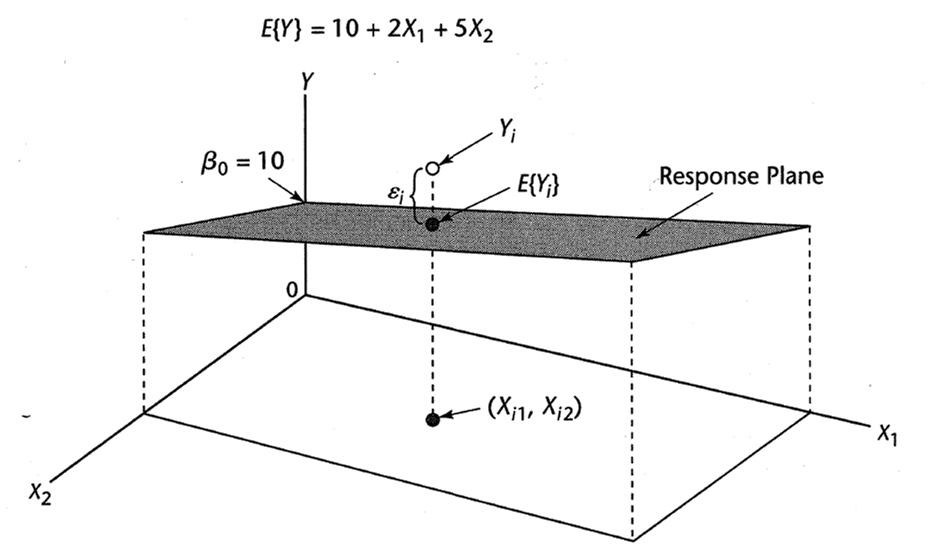
\includegraphics[scale=.4]{26.png}
 \end{figure}

}

\frame[t] {
 \frametitle{Meaning of Regression Coefficients}
 \begin{itemize}
 \item $\beta_0$ is the intercept when both $X_1$ and $X_2$ are
 zero;
 \item $\beta_1$ indicates the change in the mean response $\Ave(Y)$ per
 unit increase in $X_1$ when $X_2$ is held constant
 \item $\beta_2$ -vice versa
 \item Example: fix $X_2=2$\\
 \[\Ave(Y)=10+2X_1+5(2)=20+2X_1 ~~~~~X_2=2\]\\
 intercept changes but clearly linear 
 \item In other words, all one dimensional restrictions of the regression surface are lines.
 \end{itemize}
}

\frame[t] {
 \frametitle{Terminology}
 1. When the effect of $X_1$ on the mean response does not depend on
 the level $X_2$ (and vice versa) the two predictor variables are
 said to have additive effects or not to interact.\\
 2. The parameters $\beta_1$ and $\beta_2$ are sometimes called
 partial regression coefficients.
}

\frame[t] {
 \frametitle{Comments}
 1. A planar response surface may not always be appropriate, but
 even when not it is often a good approximate descriptor of the
 regression function in "local" regions of the input space\\
 2. The meaning of the parameters can be determined by taking
 partials of the regression function w.r.t. to each.
}

\frame[t] {
 \frametitle{First order model with $>2$ predictor variables}
Let there be $p-1$ predictor variables, then \\
\[Y_i=\beta_0+\beta_1X_{i1}+\beta_2
X_{i2}+...+\beta+{p-1}X_{i,p-1}+\epsilon_i\]
which can also be written as \\
\[Y_i=\beta_0+\displaystyle\sum_{k=1}^{p-1}\beta_k
X_{ik}+\epsilon_i\]
and if $X_{i0}=1$ is also can be written as\\
\[Y_i=\displaystyle\sum_{k=1}^{p-1}\beta_k X_{ik}+\epsilon_i\] where
$X_{i0}=1$

}

\frame[t] {
 \frametitle{Geometry of response surface}
 \begin{itemize}
 \item In this setting the response surface is a hyperplane
 \item This is difficult to visualize but the same intuitions hold\\
\begin{itemize}
\item  Fixing all but one input variables, each $\beta_p$ tells how much the
 response variable will grow or decrease according to that one input variable
\end{itemize}

 \end{itemize}

}


\frame[t] {
 \frametitle{General Linear Regression Model}
 We have arrived at the general regression model. In general the
 $X_1,...,X_{p-1}$ variables in the regression model do not have to
 represent different predictor variables, nor do they have to all be
 quantitative(continuous).
 \bigskip
 
 The general model is \\
 \begin{center}
 $Y_i=\displaystyle\sum_{k=1}^{p-1}\beta_k X_{ik}+\epsilon_i$ where
 $X_{i0}=1$
 \end{center}
 with response function when $\Ave(\epsilon_i)$=0 is

\[\Ave(Y)=\beta_0+\beta_1 X_1+...+\beta_{p-1}X_{p-1}\]
 }








\end{document}
